\section{Results and Analysis}
\subsection{Variables selection}
\subsubsection{Correlations}
We aim to analyse our datasets because we have too many variables (21 for PEPSI and 41 for Hydroswot). We need to reduce this number and to focus only on the essential variables. We make an advanced descriptive analysis.\\

First, we calculate correlations. 
\begin{figure}[H]
\centering
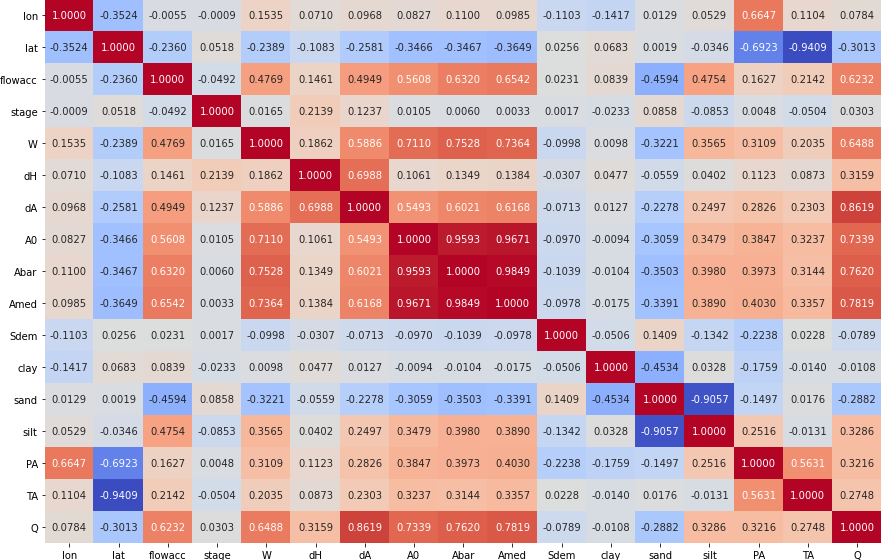
\includegraphics[scale=0.4]{Graph/correlation_hydro.png}
\caption{Correlation in HydroSwot dataset}
\label{corH}
\end{figure}

For HydroSwot, we can see in figure~\ref{corH} that the highest coefficients of correlation with $Q$ are $dA$, $W$,$flowacc$, $A0$, $Abar$ and $Amed$. It makes sense to see $A0$, $Abar$ and $Amed$ so high because they are part of the equation to compute $Q$. On the other hand, $dA$, $W$, and $flowacc$ appear to be variables the most correlated with $Q$. In contrast, $Sdem$ is not highly correlated with $Q$.
\begin{figure}[H]
\centering
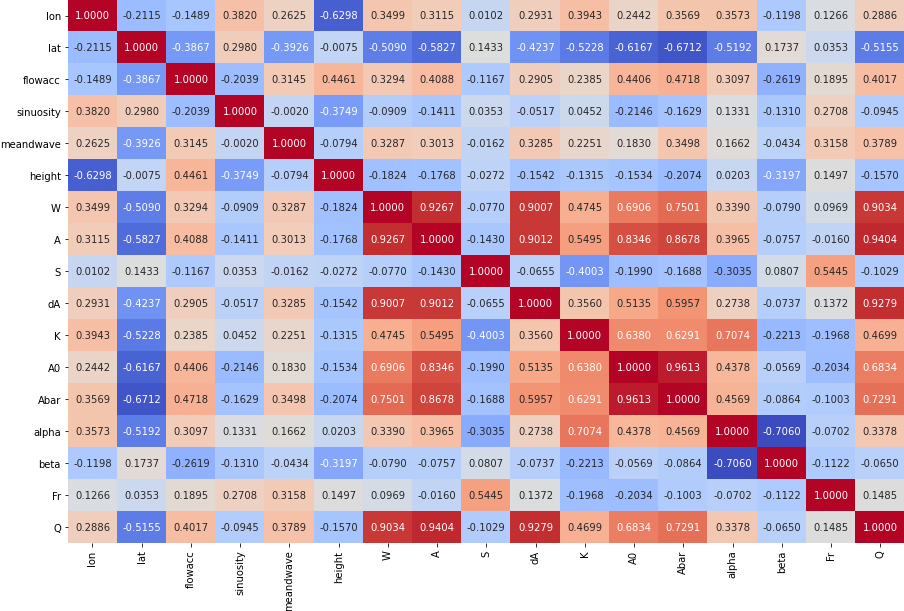
\includegraphics[scale=0.4]{Graph/correlation_pepsi.png}
\caption{Correlation in Pepsi dataset}
\label{fig:tab2}
\end{figure}

For Pepsi, we calculate the correlation in figure \ref{fig:tab2}. We make the same observations as for Hydrowswot. In addition, we can see the high correlation coefficient of the Strickler coefficient. 

To conclude the analysis of the correlation coefficients, the most essential variables that explain $Q$ seem to be $flowacc$, $W$ and $dA$.$Sdem$ We want to verify this conclusion and then do a principal component analysis. 

\subsubsection{Principal Component Analysis}

 Firt step of a PCA is to determine the number of principal components. Due to the high dimension of our datasets, boxplot of the components is hardly sufficient to determine a good number. 
 
 \begin{figure}[H]
     \centering
     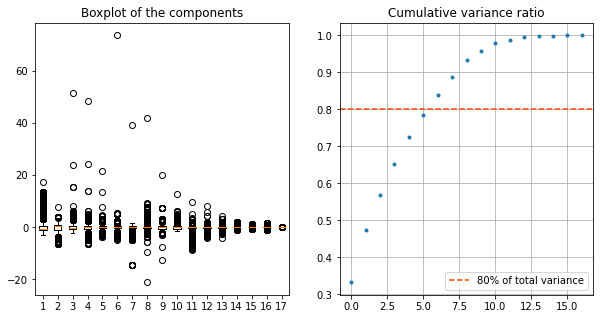
\includegraphics[scale = 0.6]{Graph/hydro_pca.png}
     \caption{HydroSwot}
     \label{fig:my_label}
 \end{figure}
 
Although we cannot determine the exact number of components through the boxplot, the plot of the cumulative variance ratio shows that 6 components are enough to reach $80\%$ of the total. 

 \begin{figure}[H]
     \centering
     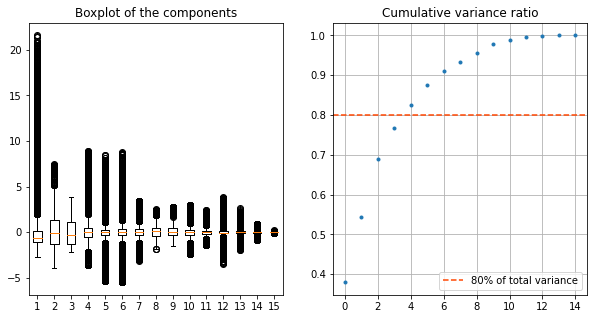
\includegraphics[scale = 0.6]{Graph/pepsi_pca.png}
     \caption{HydroSwot}
     \label{fig:my_label}
 \end{figure}

For Pepsi, 4 components seem to be sufficient. The last components represent a small ratio of variance, so we study the two first and most important of them. 


 \begin{figure}[H]
     \centering
     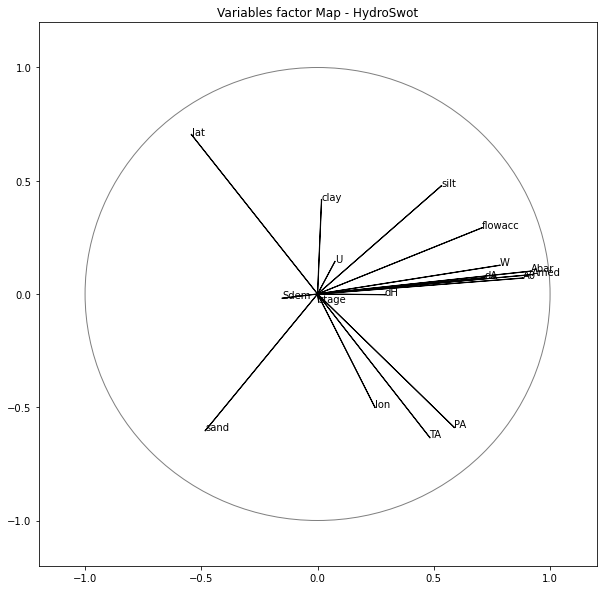
\includegraphics[scale = 0.3]{Graph/factor_map_hydro.png}
     \caption{HydroSwot}
     \label{fig:my_label}
 \end{figure}


As we can see, for HydroSwot, the variables that most explain both the first and second components are $flowacc$, $dA$ and $W$. We also notice the importance of the composition of the river with $sand$ and $silt$, the meteorological data with $PA$ and $TA$ and finally the geographical position. 



 \begin{figure}[H]
     \centering
     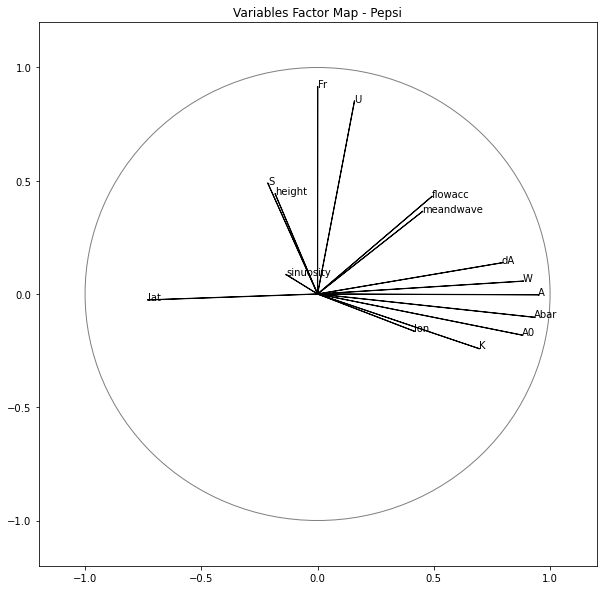
\includegraphics[scale = 0.3]{Graph/factor_map_pepsi.png}
     \caption{HydroSwot}
     \label{fig:my_label}
 \end{figure}

As for HyrdoSwot, $flowacc$, $dA$ and $W$ are good descriptors of the components. This time, we observe a good importance of the slope $S$. We can therefore think of using it as an input variable for neural networks. Once again, we observe the importance of the physical metric such as the Froude Number, $Fr$, and the Strickler coefficient, $K$. 

To  summarise, the multidimensional analysis leads us to use as input variables for neural networks : $flowacc$, $W$, $dA$ and the slope ( $S$ for Pepsi and $Sdem$ for HydroSwot). 

\subsection{River Classification} 

To have the most accurate flow estimation, we split rivers into groups. We need to define the number of groups and how to determine them. \\

We compute a k-means classification for the two datasets with 2 and 3 groups. More groups would lead to too small groups i.e. with not enough observations to run neural networks algorithms. \\
For both datasets, the k-means classification on 2 groups determines a huge group with almost the majority of the observations and the other with the rest of the observations. The k-means classification with 3 groups leads to 2 equivalent groups in size and the third group remains small.\\

Figure \ref{fig:kmeans} shows a representation of classes by k-means for the Hydroswot database. We notice that k-means separate groups distinctly. We determine that observations of the same river can be in several groups. k-means classification does not separate rivers between them. It suggests to separate data by river portions.
\begin{figure}[H]
    \begin{subfigure}{0.45 \textwidth}
        \centering
        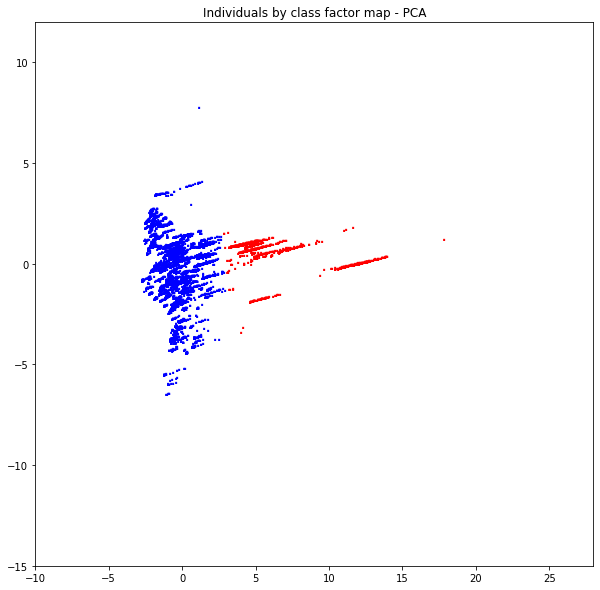
\includegraphics[scale = 0.35]{Graph/kmeans2HS.png}
        \caption{2 classes}
    \end{subfigure}
\centering
    \begin{subfigure} {0.45 \textwidth}
        \centering
        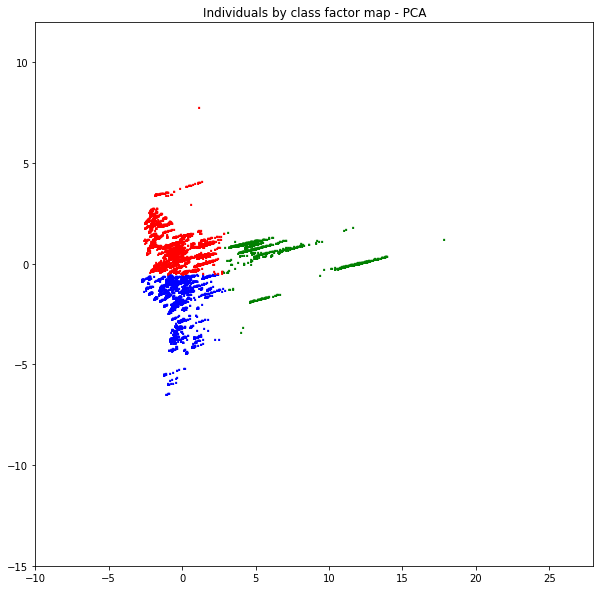
\includegraphics[scale = 0.35]{Graph/kmeans3HS.png}
        \caption{3 classes}
    \end{subfigure}
\caption{Plots for different numbers of classes in the plan of the 2 first ACP components for Hydroswot }
\label{fig:kmeans}
\end{figure}




We examine boxplots of the different variables depending of groups determined by k-means for both datasets. With 2 groups, $Q$, $dA$ and $flowacc$ are good separators. $Flowacc$ is also a good separator for 3 groups. 

\textit{boxplot Q , flowacc 2 classes et flowacc 3 classes pour hydroswot et pour pepsi}


We choose two ways to separate rivers for both datasets. Each methods separate rivers into 2 groups. We do not have enough data to create 3 groups. \\
First, we group data by rivers and compute the river flow mean. We separate them using the criteria of $Q$ which is a good separator according to k-means method. For Hydroswot, we make 2 groups: High river flow ($Q > 1000 m^3/s$) and Low river flow ($Q < 1000 m^3/s$). For Pepsi we fix the boundery at $3000 m^3/s$. We notice that the high river flow group for PEPSI contains only 3 rivers: Mississipi, Padma and Jamuna. This separation by entire rivers is close to the real context of the SWOT Mission. For neural networks algorithms, we will train and test on entire rivers that we know exactly. Then, we will use this algorithm on unknown rivers that the satellite would have measured. We name these separations Handmade Hydroswot/PEPSI Low/High $Q$. 

On the contrary, the second way to separate data is by observation. We follows k-means method to split Hydroswot and Pepsi into 2 classes. Among separative variables we have $Q$, we decide to name the two classes with Low $Q$ and High $Q$.  \\
Figure 
\begin{table}[H]
\centering
    \begin{tabular}{|c|c|c|}
    \hline
    & Low $Q$ & High $Q$ \\ \hline
    Handmade Hydroswot & 6714 & 5129 \\\hline
    Handmade Pepsi & 47548 & 3721 \\\hline
    Hydroswot k-means  &  10490 & 1140 \\\hline
    Pepsi k-means & 47536 & 2674\\ \hline
    \end{tabular}

\caption{Class size}
\label{Tab:Proportion of observations in classes}
\end{table}

Table \ref{Tab:Class size} shows the proportion of observations according to the class and the dataset. We notice that Hydroswot k-means high $Q$ has only 1140 observations. This small number may impact the efficiency of neural networks. 

\subsection{Neural Networks training ANN}

\subsubsection{Data preparation}

As explained in the previous part, we separate our datasets in classes. These classes are defined by k-means or by hand on full river or not. Handmade full river corresponds to a separation in train and test set by full rivers and not by observations. Hence, we compute several neural networks on following databases : \\
-- Hydroswot k-means low Q \\
-- Hydroswot k-means high Q \\
-- PEPSI k-means low Q \\
-- PEPSI k-means high Q \\
-- Handmade Hydroswot low Q full river \\
-- Handmade Hydroswot high Q full river\\
-- Handmade PEPSI low Q full river \\
-- Handmade PEPSI high Q full river \\
-- Handmade Hydroswot low Q  \\
-- Handmade Hydroswot high Q\\
-- Handmade PEPSI low Q  \\
-- Handmade PEPSI high Q \\

Each database is randomly separate in train and test sets with proportion 80\% and 20\% respectively. We have to notice that these proportions are not exactly respected for handmade full river databases. This is due to the constraint of extracting full rivers from the initial database. 

\subsubsection{Architecture}

Before training neural networks, we must decide of its architectures. First, we need to determine the number of layers and the number of neurons in each layer. These parameters depending on the shape of the data we will train the ANN with, the architecture is different in function of the database. 

A large data set such as handmade PEPSI high Q will require an ANN with more layers and neurons than a data set like hydroswot k-means high $Q$. To determine the best architecture, we build several neural networks for each database, and compare their efficiency through different metrics : Mean Squared Error and Mean Absolute Error.

As a result, we choose for PEPSI low Q databases a neural network with 32 layers containing 32 neurons. We choose 8 layers and 8 neurons in each for PEPSI high Q databases. For hydroswot databases, we choose a 8x8 or 16x16 neural network depending on the size. We aim to have more data in the training set than the number of parameter in the neural network.

Regarding the parameters of the ANN, 100 epochs is enough for the algorithm to converge. We choose a batch size of 25.

We use the mean square error (mse) as loss function. 

\subsubsection{Training}

To estimate the goodness of fit of the neural network, we use two different metrics.We plot the results. We aim to observe a convergence.  Here, figure \ref{fig:metricANN} shows the results, on the HydroSwot  Handmade High Q class.

\begin{figure}[H]
    \begin{subfigure}{0.45 \textwidth}
        \centering
        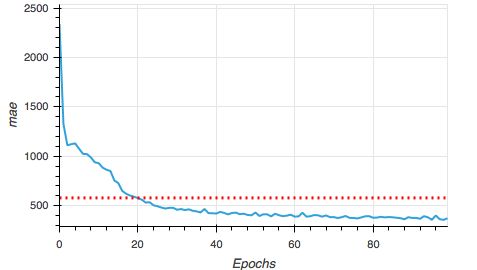
\includegraphics[scale = 0.45]{Graph/MAE_hydroHQ.png}
        \caption{Mean Absolute Error}
       
    \end{subfigure}
    \centering
     \begin{subfigure}{0.45 \textwidth}
         \centering
        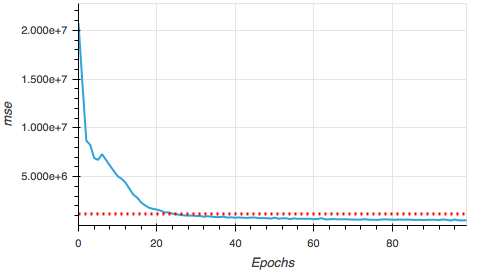
\includegraphics[scale = 0.45]{Graph/MSE_hydroHQ.png}
        \caption{Mean Square Error}
       
     \end{subfigure}
 
 \caption{Goodness of fit of the neural network, Handmade HydroSwot High Q}
 \label{feig:metricANN}
\end{figure}

We observe that the two curves decrease suddenly during the $20$ first epochs, and then much more slowly to finally converge below the $20\%$ error limit. In that case, the goodness of fit of the neural network is pretty good. We also observe it on the graph below, where we see the hydrograph of a river taken from the train set.

- hydrograph prediction on a river from the train set \\


\subsubsection{Testing}

After the training of our neural network, we evaluate its performances. Thus, we use the test set - not used during the training - to predict river discharge. As mentioned before, we plot the predictions against the real values. On the graph below, our predictions are computed on the \textbf{Name of set}.

\begin{figure}[H]
    \centering
    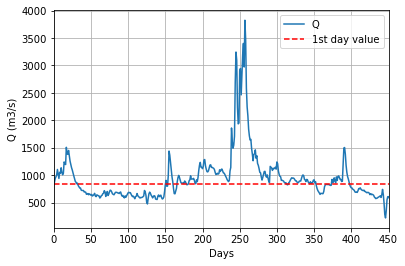
\includegraphics[scale = 0.5]{Graph/1year.png}
    \label{fig:my_label}
    \caption{ANN test set predictions, \textbf{Name of set}}
\end{figure}

We observe...

Then, in order to focus on the predictions of a river in particular, we plot the predicted hydrographs of the rivers of the test set, and we compare them to their true measures. Here, the following hydrograph is the one of \textbf{Name of the river + which dataset it comes from}.

\begin{figure}[H]
    \centering
    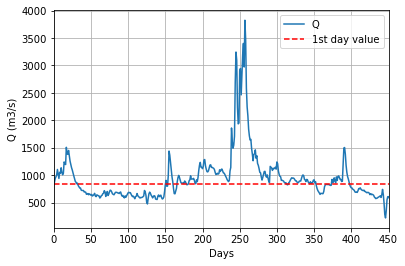
\includegraphics[scale = 0.5]{Graph/1year.png}
    \label{fig:my_label}
    \caption{Hydrograph, \textbf{Name of river and name of set}}
\end{figure}

We observe...

Finally, to quantify precisely the errors of the model, we compute the different metrics mentioned in section $x.y$.\newline

\textbf{Table of results. Monte Carlo like or not ?}
 
\subsection{Neural Networks training LSTM}

\subsubsection{Data preparation}
LSTM neural networks are based on time series. Hence, we can only use the Pepsi data set where the variable $day$ is present. The measurement sequences available in PEPSI goes from 145 days to a maximum of 595 days. LSTM neural networks learn from a single river time serie. Therefore, the sequences we have are too small. We need to periodise the time series over several years to obtain a sufficiently large data set and a pattern that repeats over the years. We assume that the river flow of a river is the same over the years. Because of this size problem, we focus our study on the \textit{Missouri Downstream} river which has observations on 595 days. We cut the measurements around 360 days, to have a full year, and also at a day close to the first day to have continuity between each year. 

\begin{figure}[H]
    \begin{subfigure}{0.45 \textwidth}
        \centering
        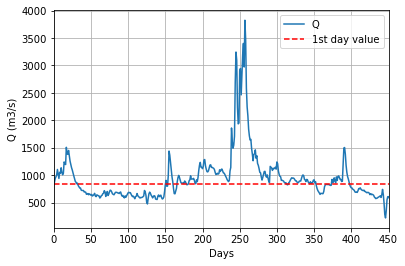
\includegraphics[scale = 0.5]{Graph/1year.png}
        \caption{1 year before}
        \label{fig:my_label}
    \end{subfigure}
    \centering
     \begin{subfigure}{0.45 \textwidth}
         \centering
        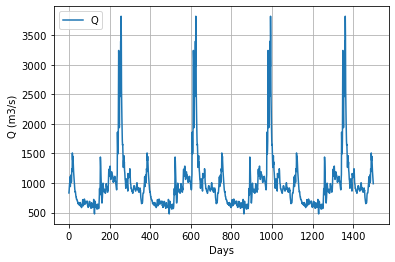
\includegraphics[scale = 0.5]{Graph/5years.png}
        \caption{5 years after periodisation}
        \label{fig:my_label}
     \end{subfigure}
 
 \caption{Periodisation of the time serie}
\end{figure}

The graph at the left shows our new dataset, ready to be used for training. We periodise on $10$ years.

\subsubsection{Parameters}

We choose 80\% - 20\% for the proportion between train and test set. We set the sequence length at 16, i.e. the number of days used to predict the next day, and the batch size to 16 also. We can say that these numbers are small, but we will see that they are enough. We make a change in the features used for the training. \textit{Flowacc} is now constant in the time serie because we consider a single river and a single reach. Thus, we put \textit{W}, \textit{dA} and \textit{S} as input data, and \textit{Q} always as output data. \\

For \textit{MissouriDownstream} river, we obtain a train set composed of 2944 days, and 736 days for the test set. We hence get 183 batches available for the training. We build a neural network with 10 LSTM cells which give us 571 trainable parameters. Mean Squared Error is set as the loss function and as a metric, as well as Mean Absolute Error and nRMSE. Finally, we run the neural networks trough $20$ \textit{epochs}. 




\subsubsection{Training}
We compute and display the metrics MAE and nRMSE through the $epochs$. 
\begin{figure}[H]
    \begin{subfigure}{0.45 \textwidth}
        \centering
        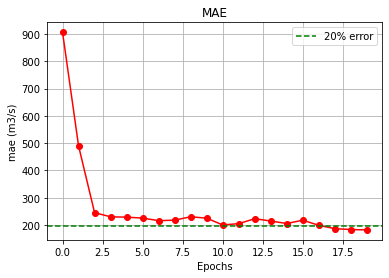
\includegraphics[scale = 0.5]{Graph/mae_lstm.png}
        \label{fig:my_label}
    \end{subfigure}
    \centering
     \begin{subfigure}{0.45 \textwidth}
         \centering
        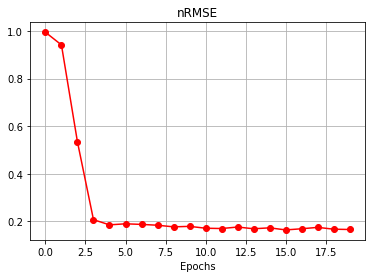
\includegraphics[scale = 0.5]{Graph/nrmse_lstm.png}
        \label{fig:my_label}
     \end{subfigure}
     \caption{Metrics}
     
\end{figure}

First, we note the decrease of both of the metrics and the beginning of their convergence from the fifth epoch. The beginning of the convergence coincides with 20\% of physical error rate. The convergence rate is the best achieved so far, and the most stable. We observe now the river flow prediction computed on the train test.

\begin{figure}[H]
    \begin{subfigure}{0.45 \textwidth}
        \centering
        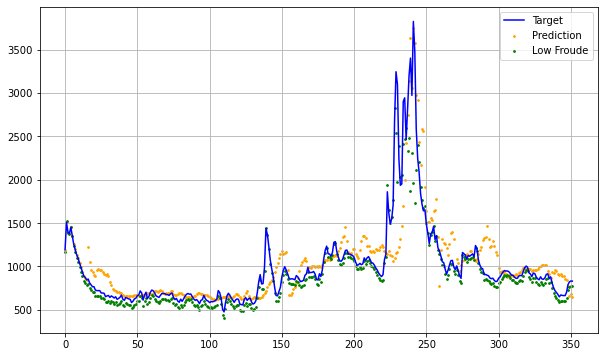
\includegraphics[scale = 0.35]{Graph/pred_low_fr_missour_lstm.png}
        \caption{Prediction according to different methods}
      
    \end{subfigure}
    \centering
     \begin{subfigure}{0.45 \textwidth}
         \centering
        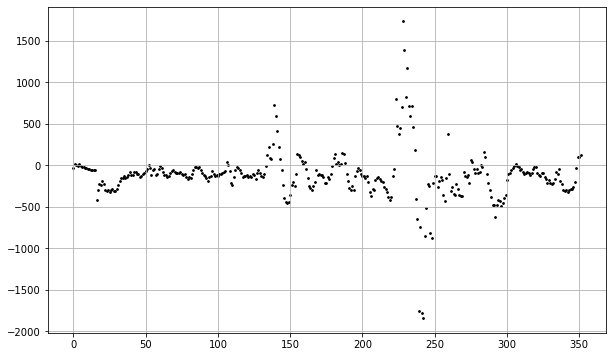
\includegraphics[scale = 0.35]{Graph/diff_lowfr_pred_lstm.png}
        \caption{Difference between low Froude and prediction}
        
     \end{subfigure}
     \caption{Results}
\label{fig: lest result} 
\end{figure}


In the figure \ref{fig: lest result}, we observe three curves close to each other. The prediction by LSTM as much as the Low-Froude model follow well the variation of the actual flow rate. Even the biggest variation peak, what we might think is a flood, is well predict, better by LSTM than by low-Froude. 

We conclude that the architecture of LSTM designed is good enough for this type of problem. The condition to obtain such results is to have enough data, and so to have enough days / years to train on. Hence, a good solution is the duplication of an existing dataset like we did. The low-Froude model also seems to be well adapted to the river. However, we observe a constant error between low-Froude and LSTM prediction. This error is strongly accentuated when it comes to the prediction of the peaks of variation. This difference is due to the difficulty of the low-Froude model to follow the biggest variations.

\subsubsection{Testing}
